\chapter[GAM]{Modelos Aditivos Generalizados}

\begin{objetivos}
	Ao final desta unidade, o estudante deverá compreender a lógica dos Modelos Aditivos Generalizados (GAM) em Modelagem de Distribuição de Espécies; ajustar modelos presença-background com suavizadores; interpretar funções suaves; avaliar desempenho preditivo por AUC, TSS, sensibilidade e especificidade; gerar curvas de resposta parcial; produzir mapas de adequabilidade ambiental para \textit{Dinizia excelsa}; e comparar a flexibilidade do GAM com o GLM da unidade anterior.
\end{objetivos}

\section{Introdução}

Os Modelos Aditivos Generalizados, ou GAMs, ampliam a estrutura dos Modelos Lineares Generalizados ao substituir parte dos termos lineares por funções suaves estimadas a partir dos dados. Em SDM, isso é particularmente útil porque as respostas das espécies aos gradientes ambientais raramente são estritamente lineares \parencite{guisan2002,guisan2017habitat,wood2017generalized}.

Enquanto o GLM exige que a forma da resposta seja especificada explicitamente, por exemplo com termos lineares e quadráticos, o GAM permite que a relação entre ocorrência e ambiente seja estimada de forma mais flexível. Assim, ele pode representar respostas unimodais, limiares, platôs e transições ambientais complexas.

\begin{equationbox}
	\[
	\text{logit}(p_i) =
	\beta_0 + f_1(x_{1i}) + f_2(x_{2i}) + \cdots + f_k(x_{ki})
	\]
\end{equationbox}

em que \(p_i\) representa a probabilidade relativa de presença no local \(i\), \(\beta_0\) é o intercepto e \(f_k(x_{ki})\) são funções suaves estimadas para cada variável ambiental.

\begin{conceito}[title={\faBook\quad GAM em SDM}]
	Em SDM, o GAM estima relações não lineares entre presença-background e variáveis ambientais por meio de funções suaves. Sua principal vantagem é a flexibilidade; sua principal cautela é evitar suavizadores excessivamente complexos que representem ruído em vez de sinal ecológico.
\end{conceito}

\section{Suavizadores e complexidade}

A flexibilidade de um GAM depende da estrutura dos suavizadores. No pacote \texttt{mgcv}, o parâmetro \(k\) define a dimensão máxima da base usada para estimar a suavização. Valores muito baixos podem produzir respostas excessivamente simples; valores muito altos podem permitir sobreajuste.

\begin{atencao}[title={\faExclamationTriangle\quad Flexibilidade não é sinônimo de qualidade}]
	Um GAM muito flexível pode capturar padrões locais dos dados de calibração, mas perder capacidade de transferência espacial ou temporal. Em SDM, a forma da curva deve ser estatisticamente adequada e ecologicamente plausível.
\end{atencao}

\section{Preparação dos dados}

Nesta unidade, utilizamos a mesma base presença-background preparada na Unidade 5 e as variáveis selecionadas após diagnóstico de multicolinearidade na Unidade 4. Isso garante continuidade metodológica entre GLM, GAM e os demais algoritmos.

\rscriptfile{scripts/unidade07/01_estrutura_pastas.R}

\rscriptfile{scripts/unidade07/02_preparar_dados_gam.R}

\section{Ajuste do GAM}

O modelo é ajustado com distribuição binomial e função de ligação logit. Cada variável ambiental selecionada entra como função suave, permitindo respostas ecológicas não lineares.

\rscriptfile{scripts/unidade07/03_ajustar_gam_dinizia.R}

\begin{figure}[H]
	\centering
	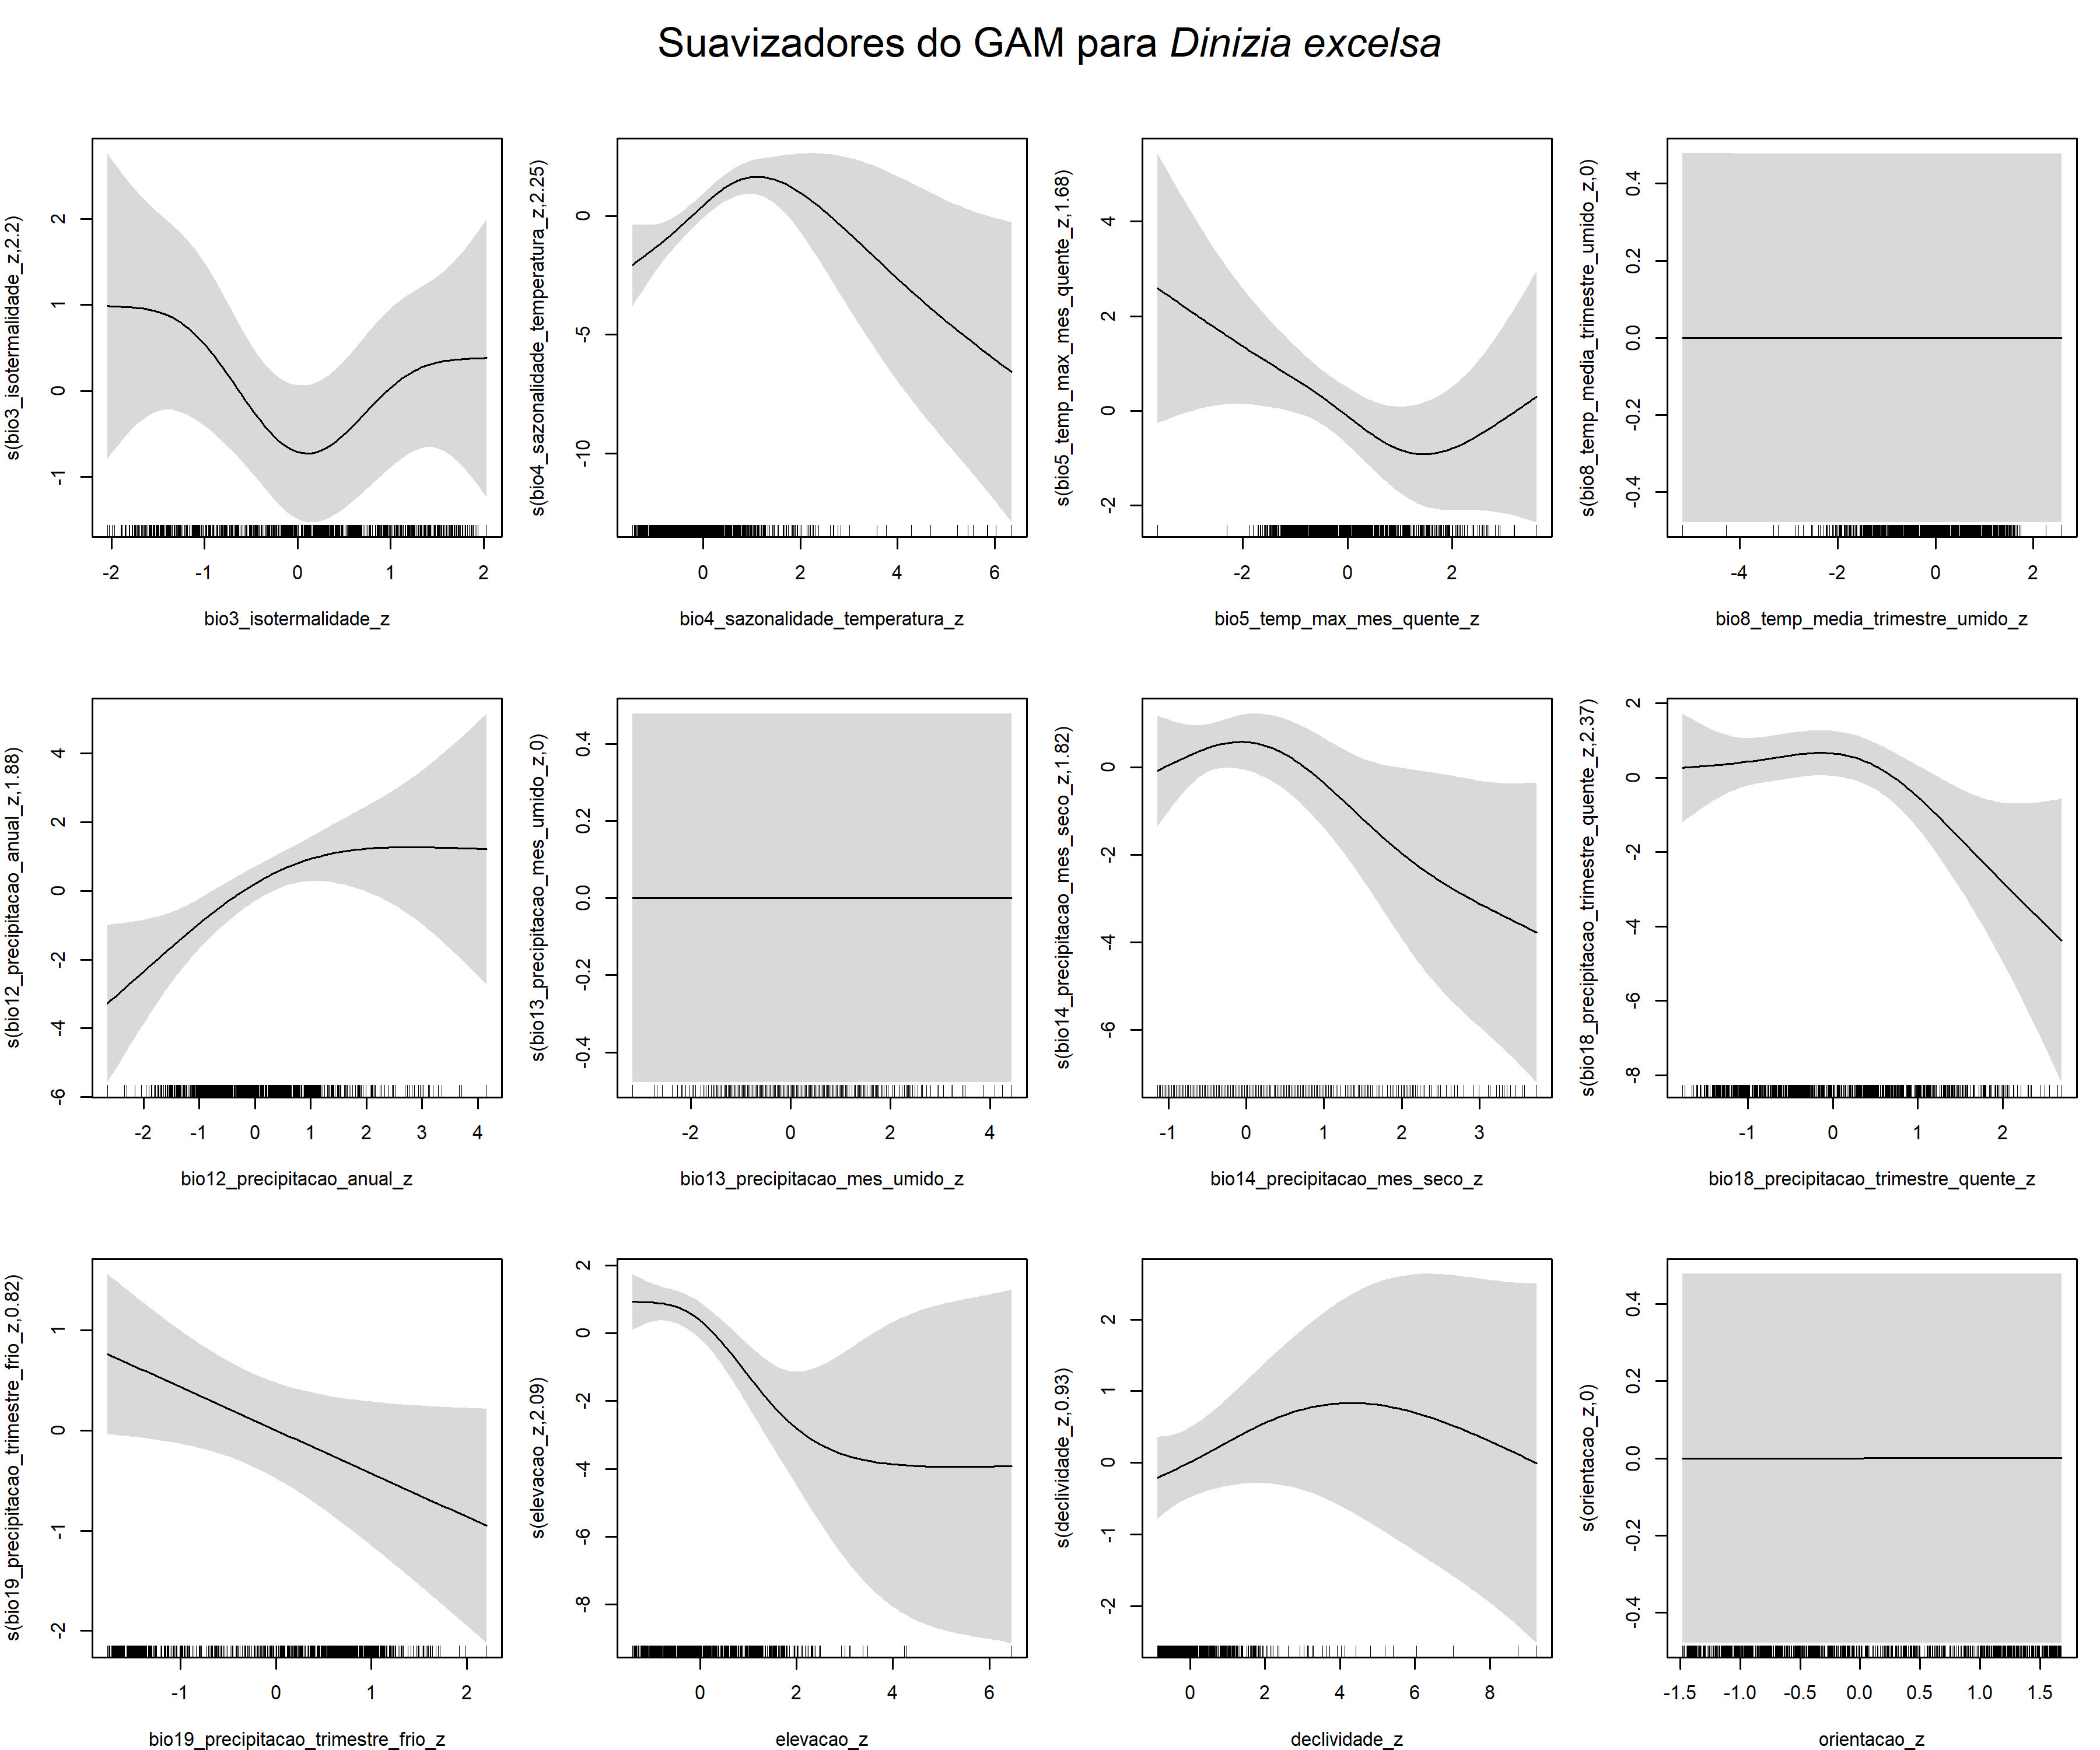
\includegraphics[width=0.96\textwidth]{figuras/unidade07/unidade07_suavizadores_gam.png}
	\caption{Funções suaves estimadas pelo GAM para as variáveis ambientais selecionadas. Cada painel representa a contribuição parcial de uma variável para a adequabilidade ambiental de \textit{Dinizia excelsa}.}
	\label{fig:unidade07_suavizadores_gam}
\end{figure}

\section{Avaliação do modelo}

O desempenho preditivo do GAM é avaliado com AUC, TSS, sensibilidade, especificidade e matriz de confusão. Essa avaliação permite comparar o GAM com o GLM ajustado na Unidade 6.

\rscriptfile{scripts/unidade07/04_avaliar_gam_dinizia.R}

\begin{figure}[H]
	\centering
	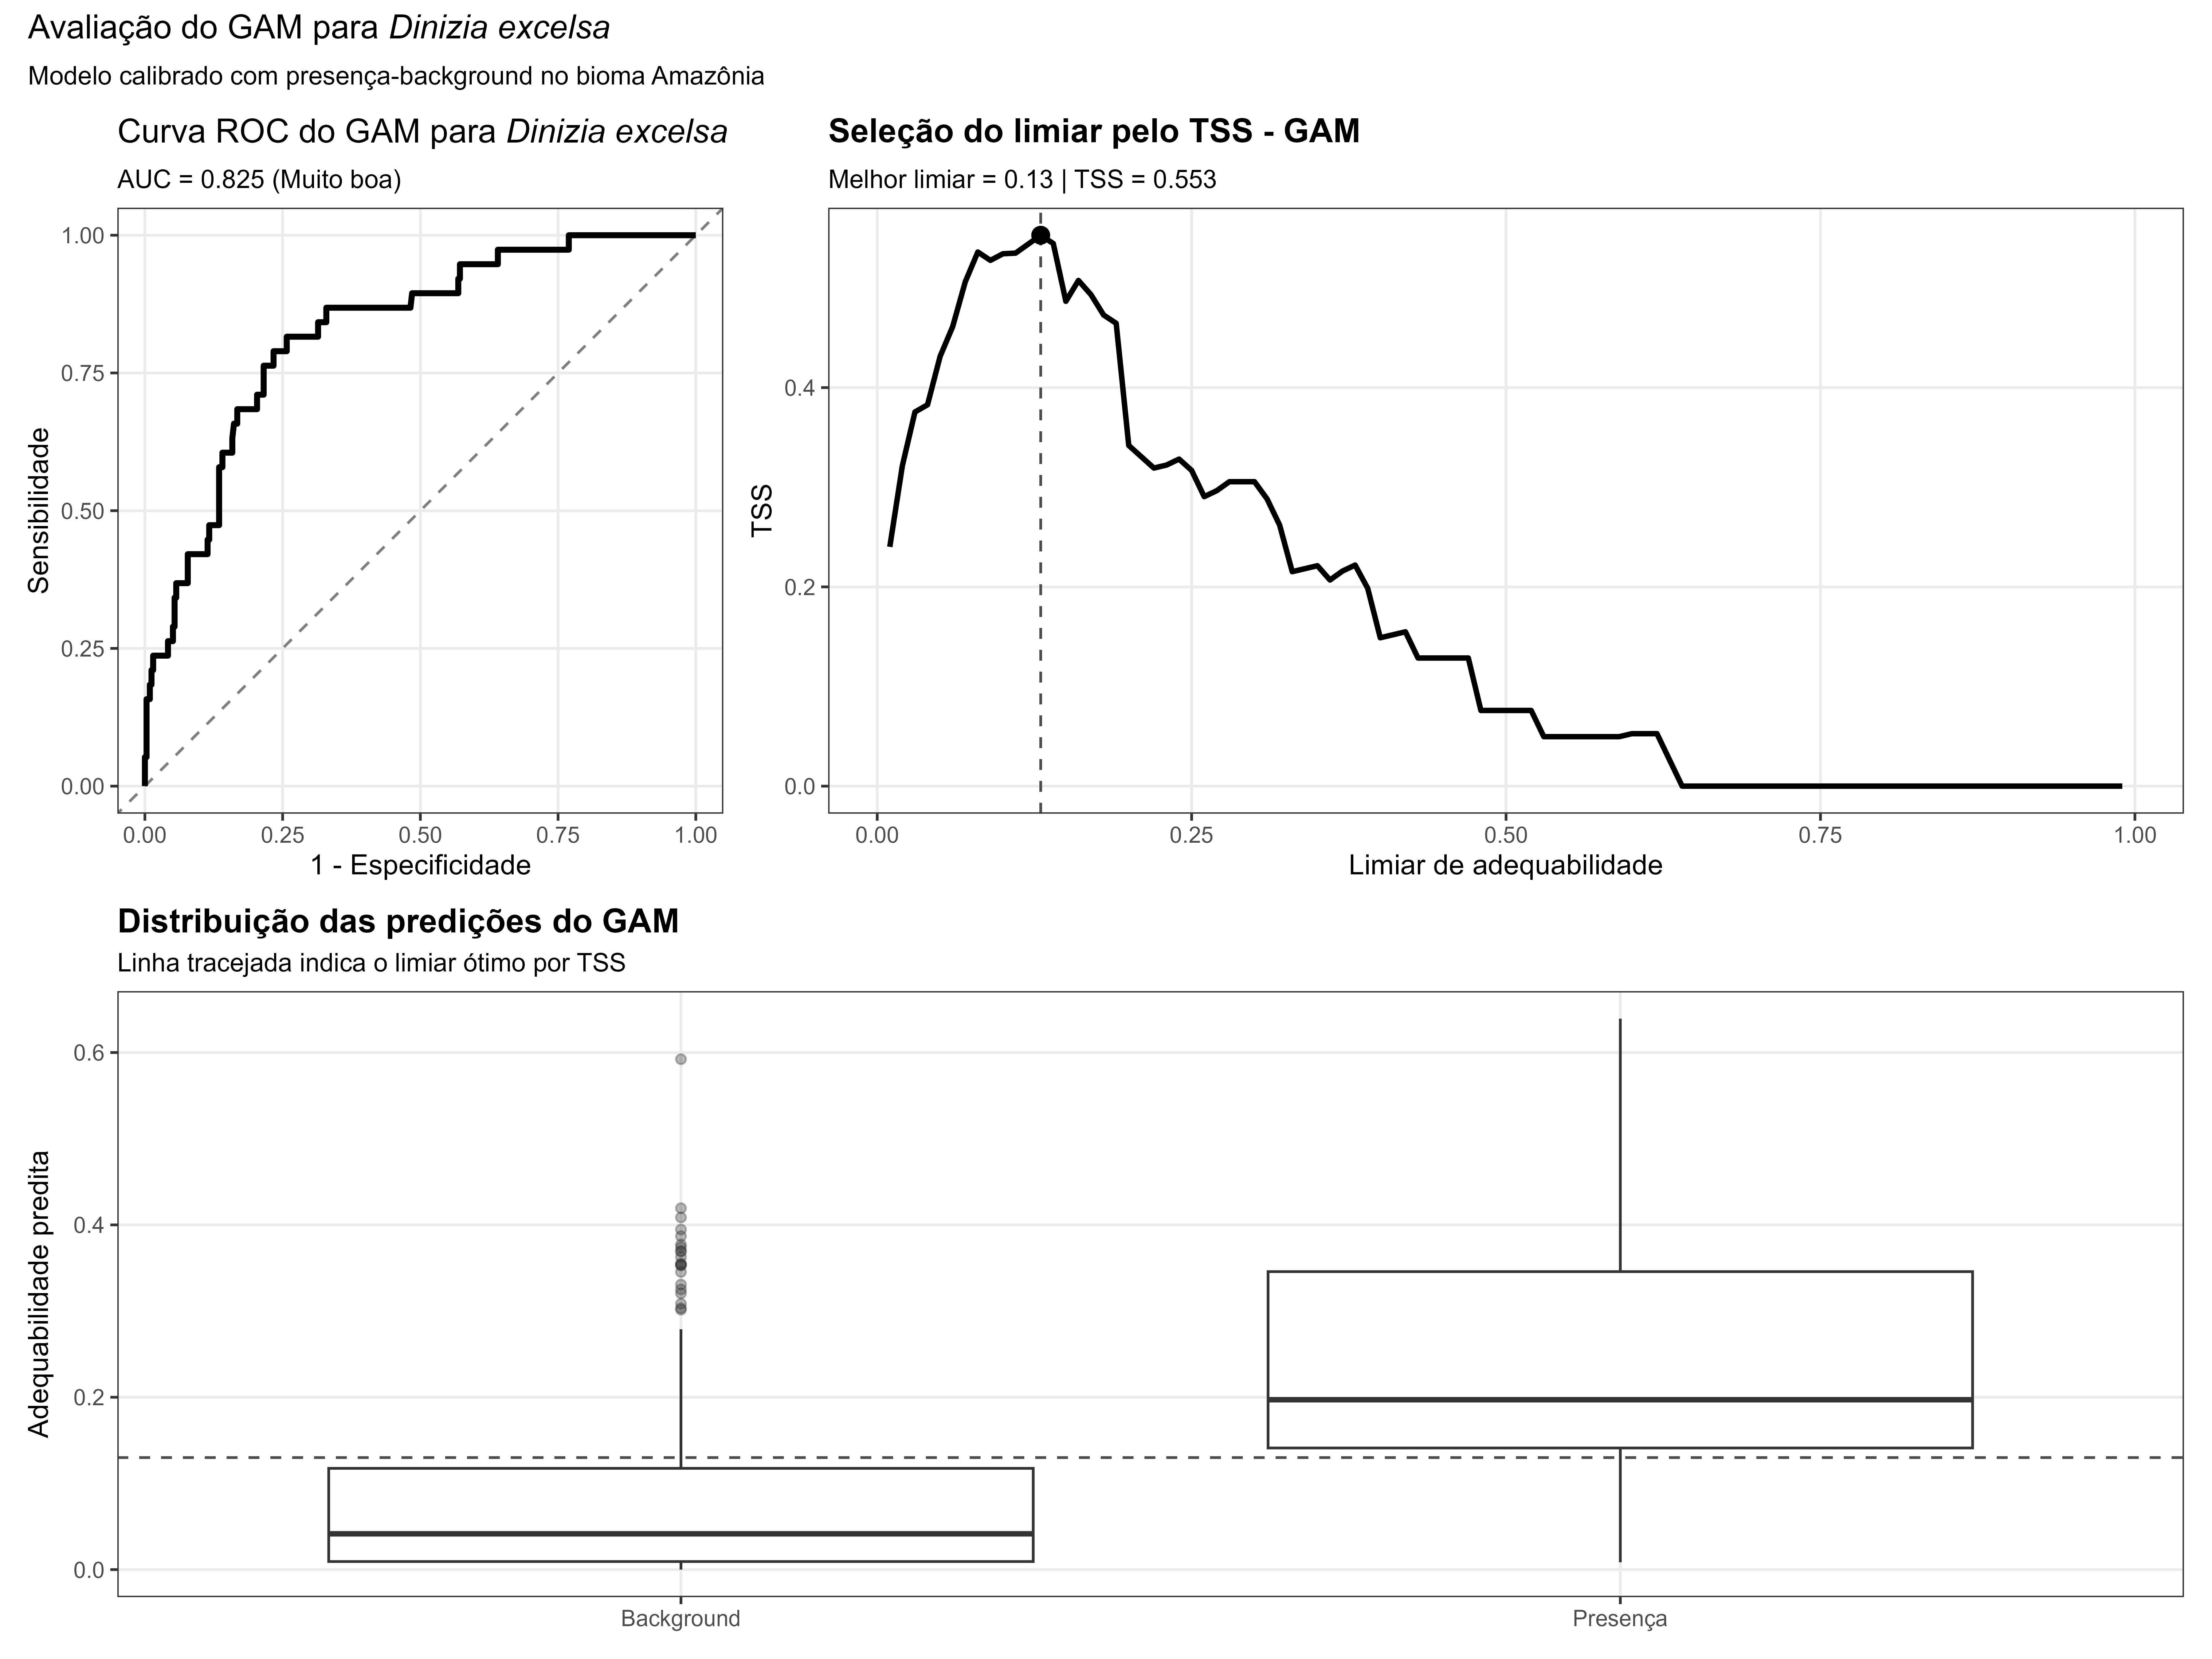
\includegraphics[width=0.78\textwidth]{figuras/unidade07/unidade07_avaliacao_gam_patchwork.png}
	\caption{Curva ROC do GAM ajustado para \textit{Dinizia excelsa}.}
	\label{fig:unidade07_roc_gam}
\end{figure}

\section{Mapa de adequabilidade atual}

O GAM é projetado espacialmente para a área acessível \(M\), gerando um mapa contínuo de adequabilidade ambiental atual.

\rscriptfile{scripts/unidade07/05_predicao_espacial_gam.R}

\begin{figure}[H]
	\centering
	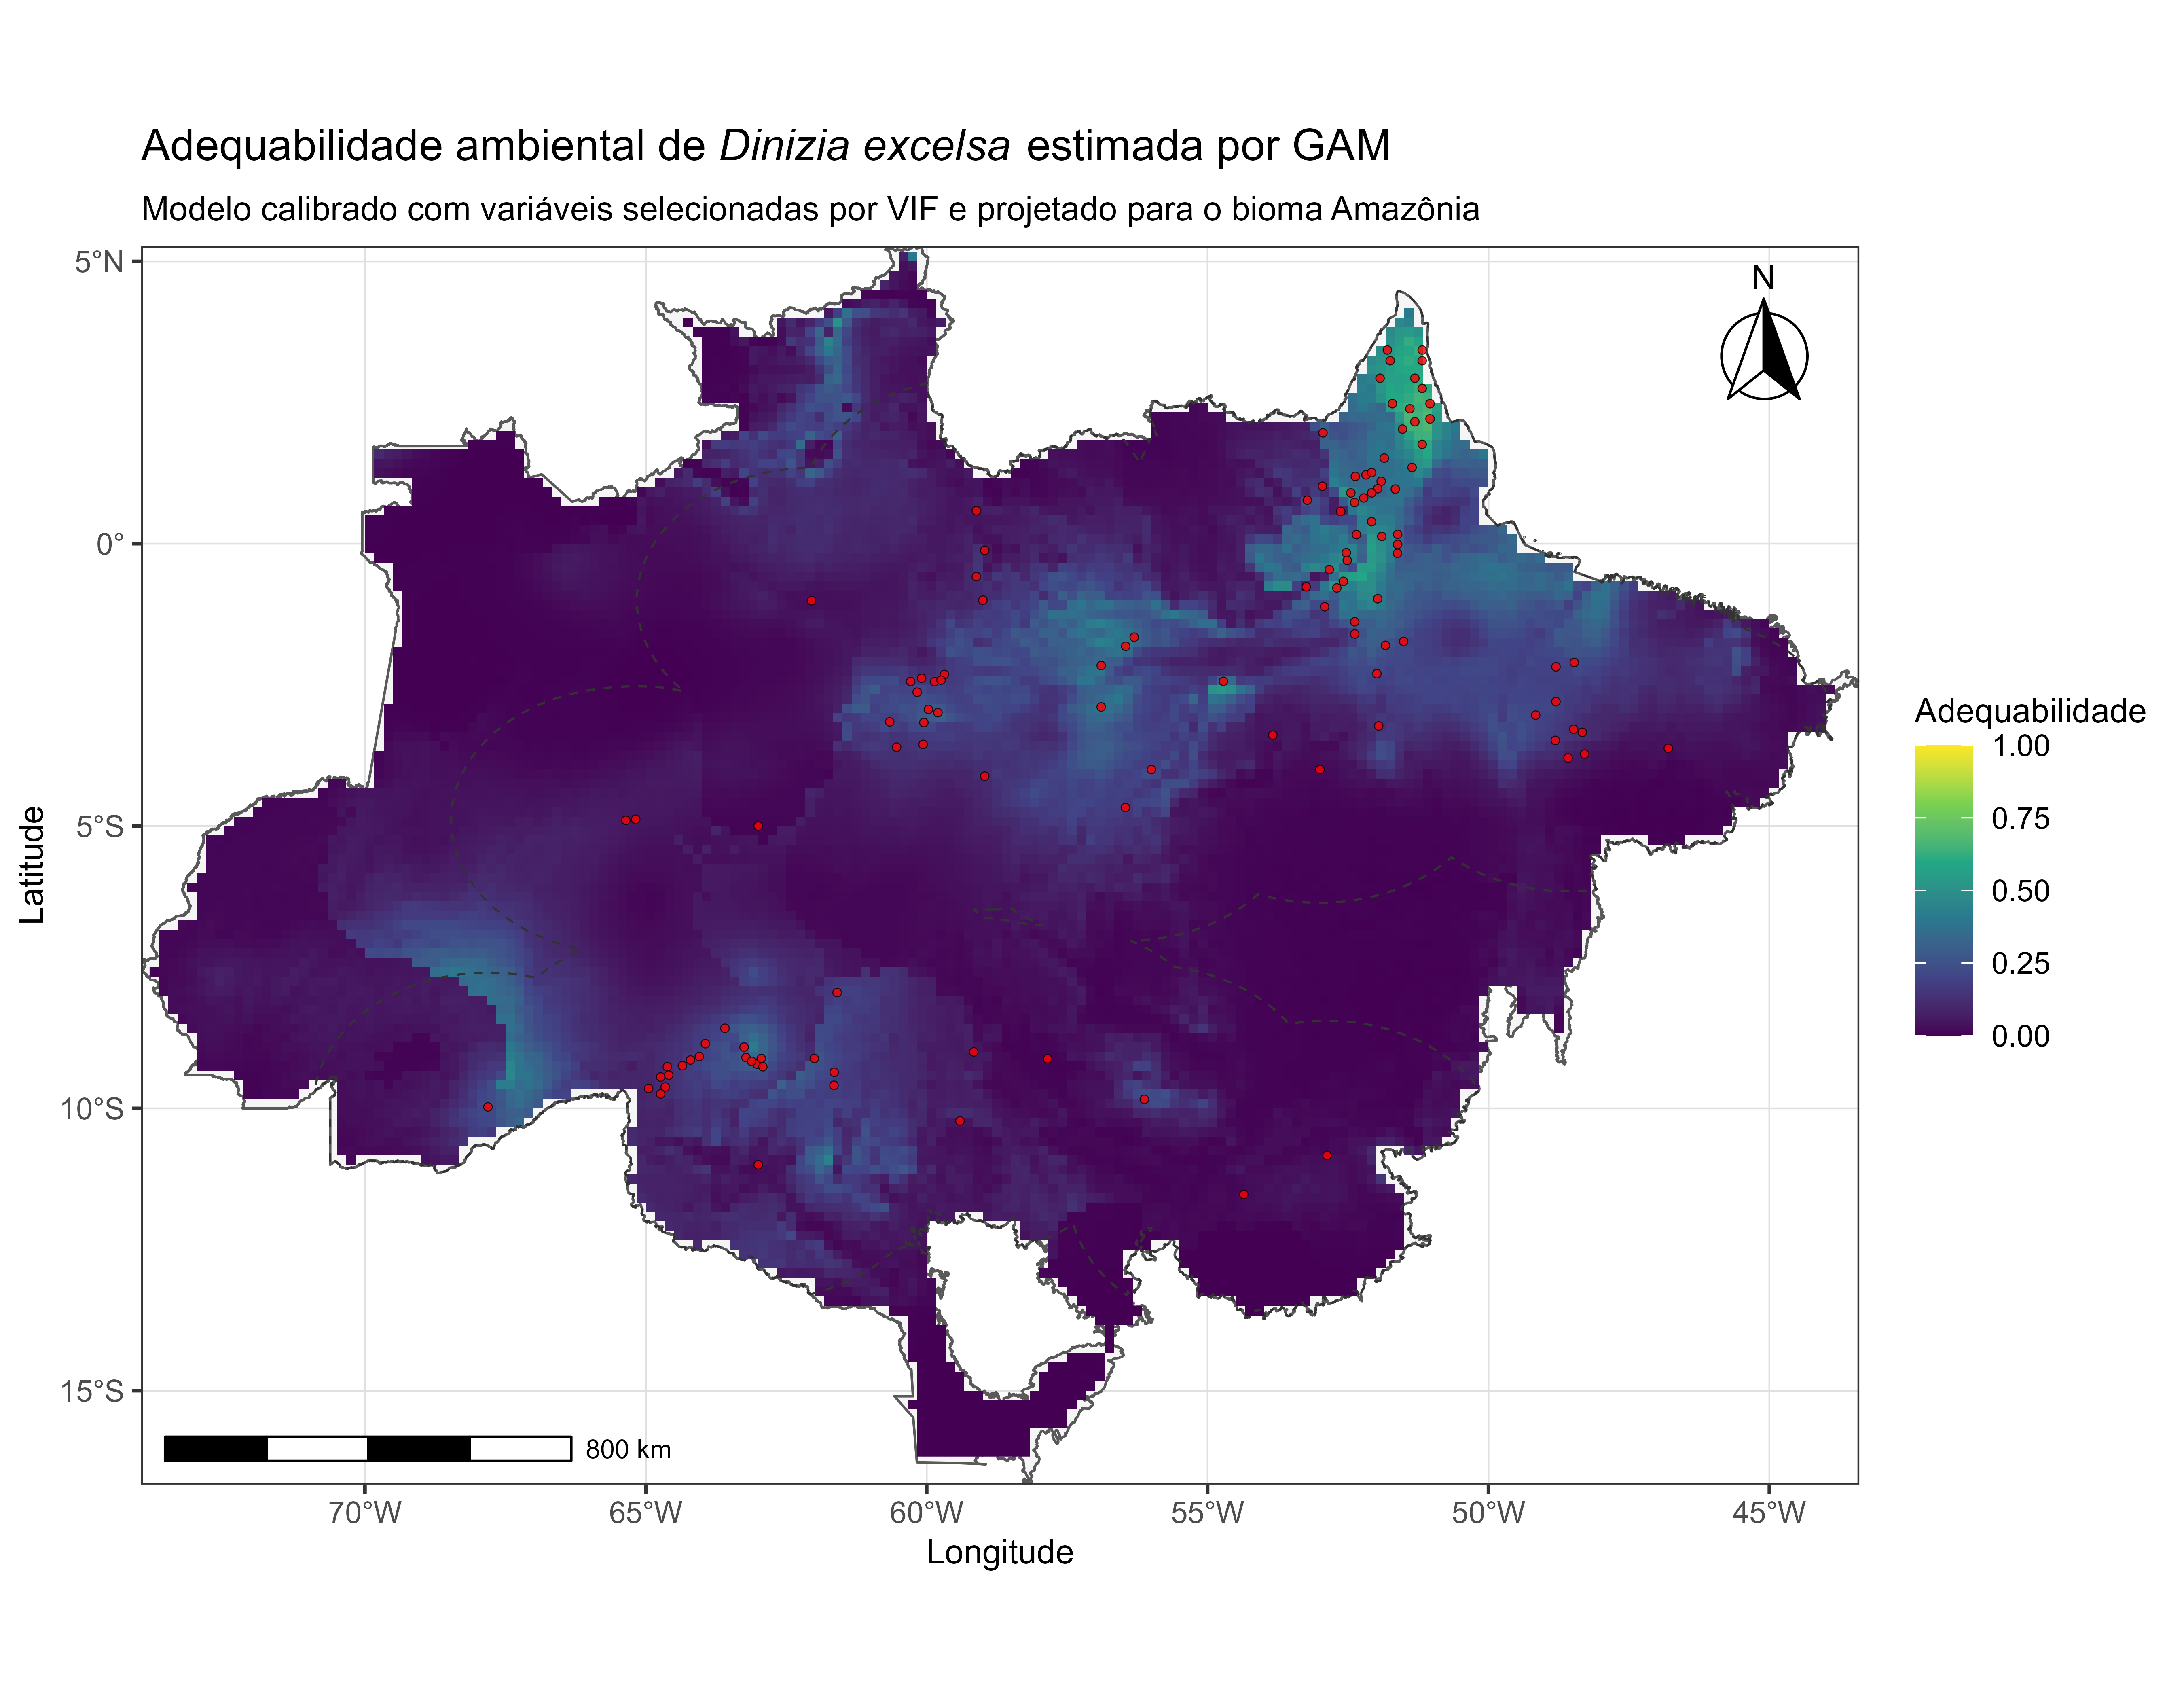
\includegraphics[width=0.88\textwidth]{figuras/unidade07/unidade07_adequabilidade_gam.png}
	\caption{Mapa de adequabilidade ambiental atual de \textit{Dinizia excelsa} estimado por GAM dentro da área acessível \(M\).}
	\label{fig:unidade07_adequabilidade_gam}
\end{figure}

\section{Curvas de resposta parcial}

As curvas de resposta parcial do GAM mostram respostas flexíveis ao longo dos gradientes ambientais, permitindo identificar faixas de maior adequabilidade, limiares e potenciais restrições climáticas.

\rscriptfile{scripts/unidade07/06_curvas_resposta_gam.R}

\begin{figure}[H]
	\centering
	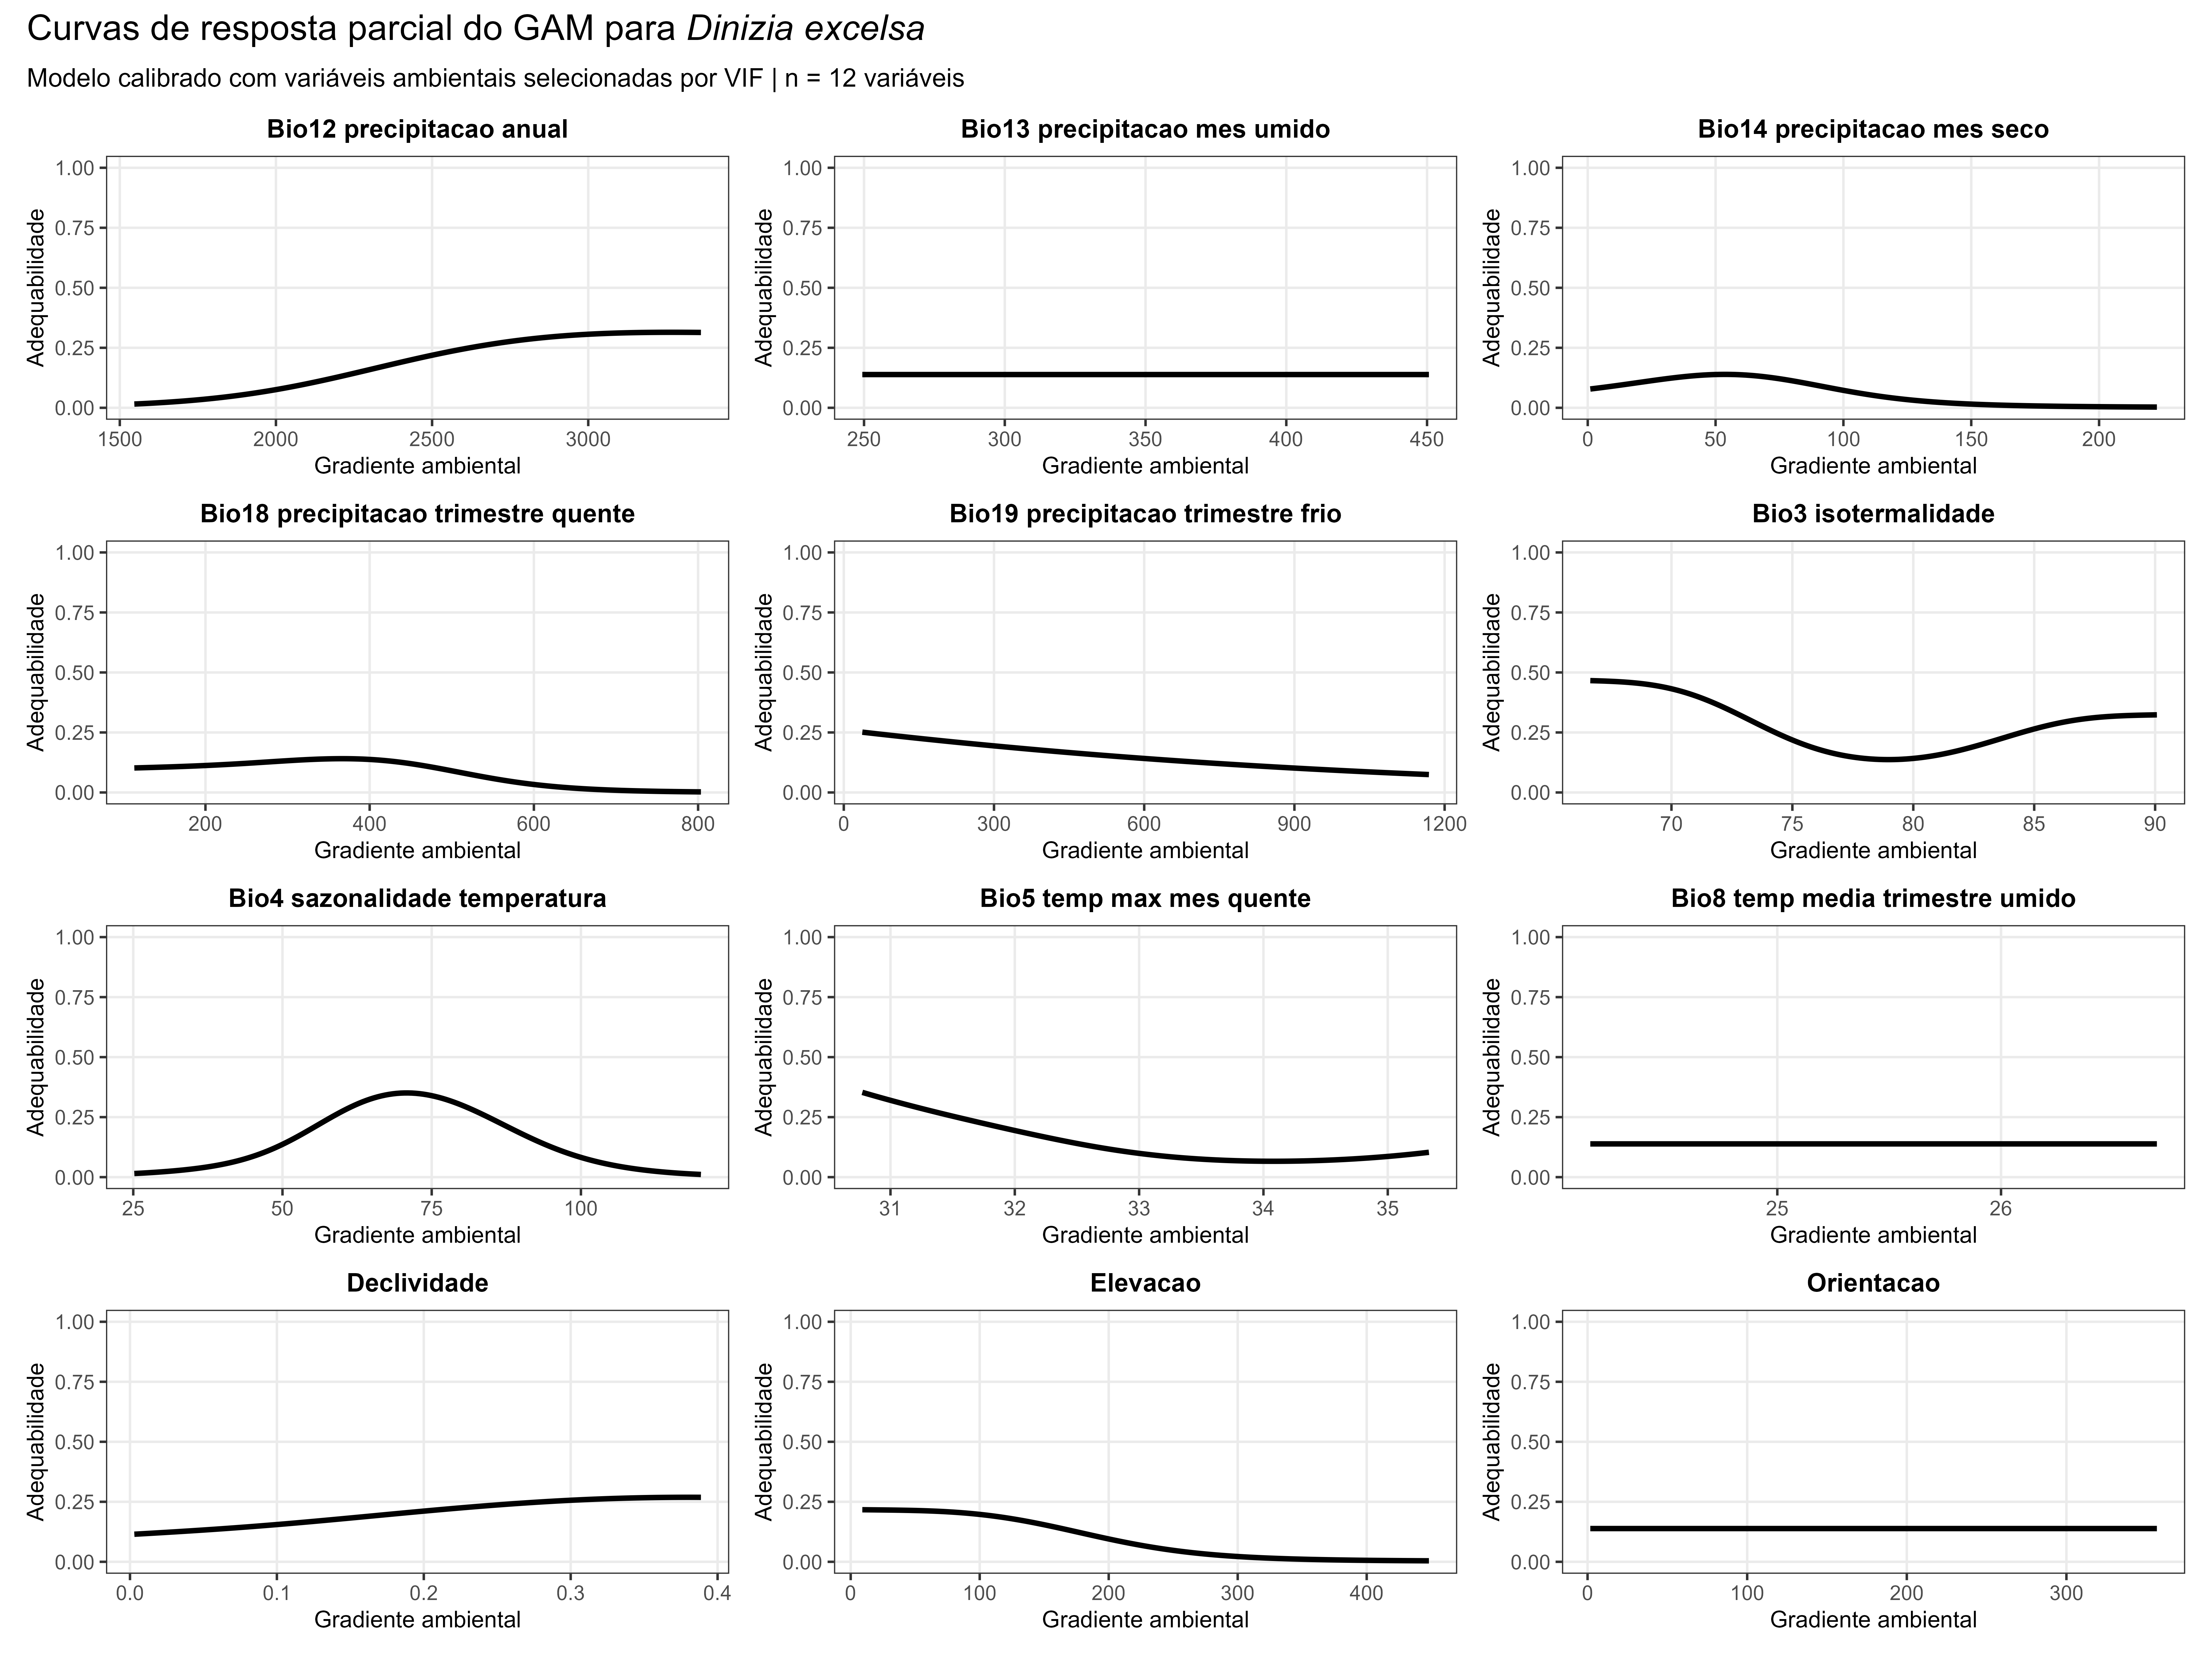
\includegraphics[width=0.96\textwidth]{figuras/unidade07/unidade07_curvas_resposta_gam.png}
	\caption{Curvas de resposta parcial do GAM para as variáveis ambientais selecionadas.}
	\label{fig:unidade07_curvas_resposta_gam}
\end{figure}

\section{Comparação entre GLM e GAM}

A comparação entre GLM e GAM permite avaliar como a maior flexibilidade do GAM altera a distribuição espacial prevista e as curvas de resposta ambiental.

\rscriptfile{scripts/unidade07/07_comparar_glm_gam.R}

\begin{figure}[H]
	\centering
	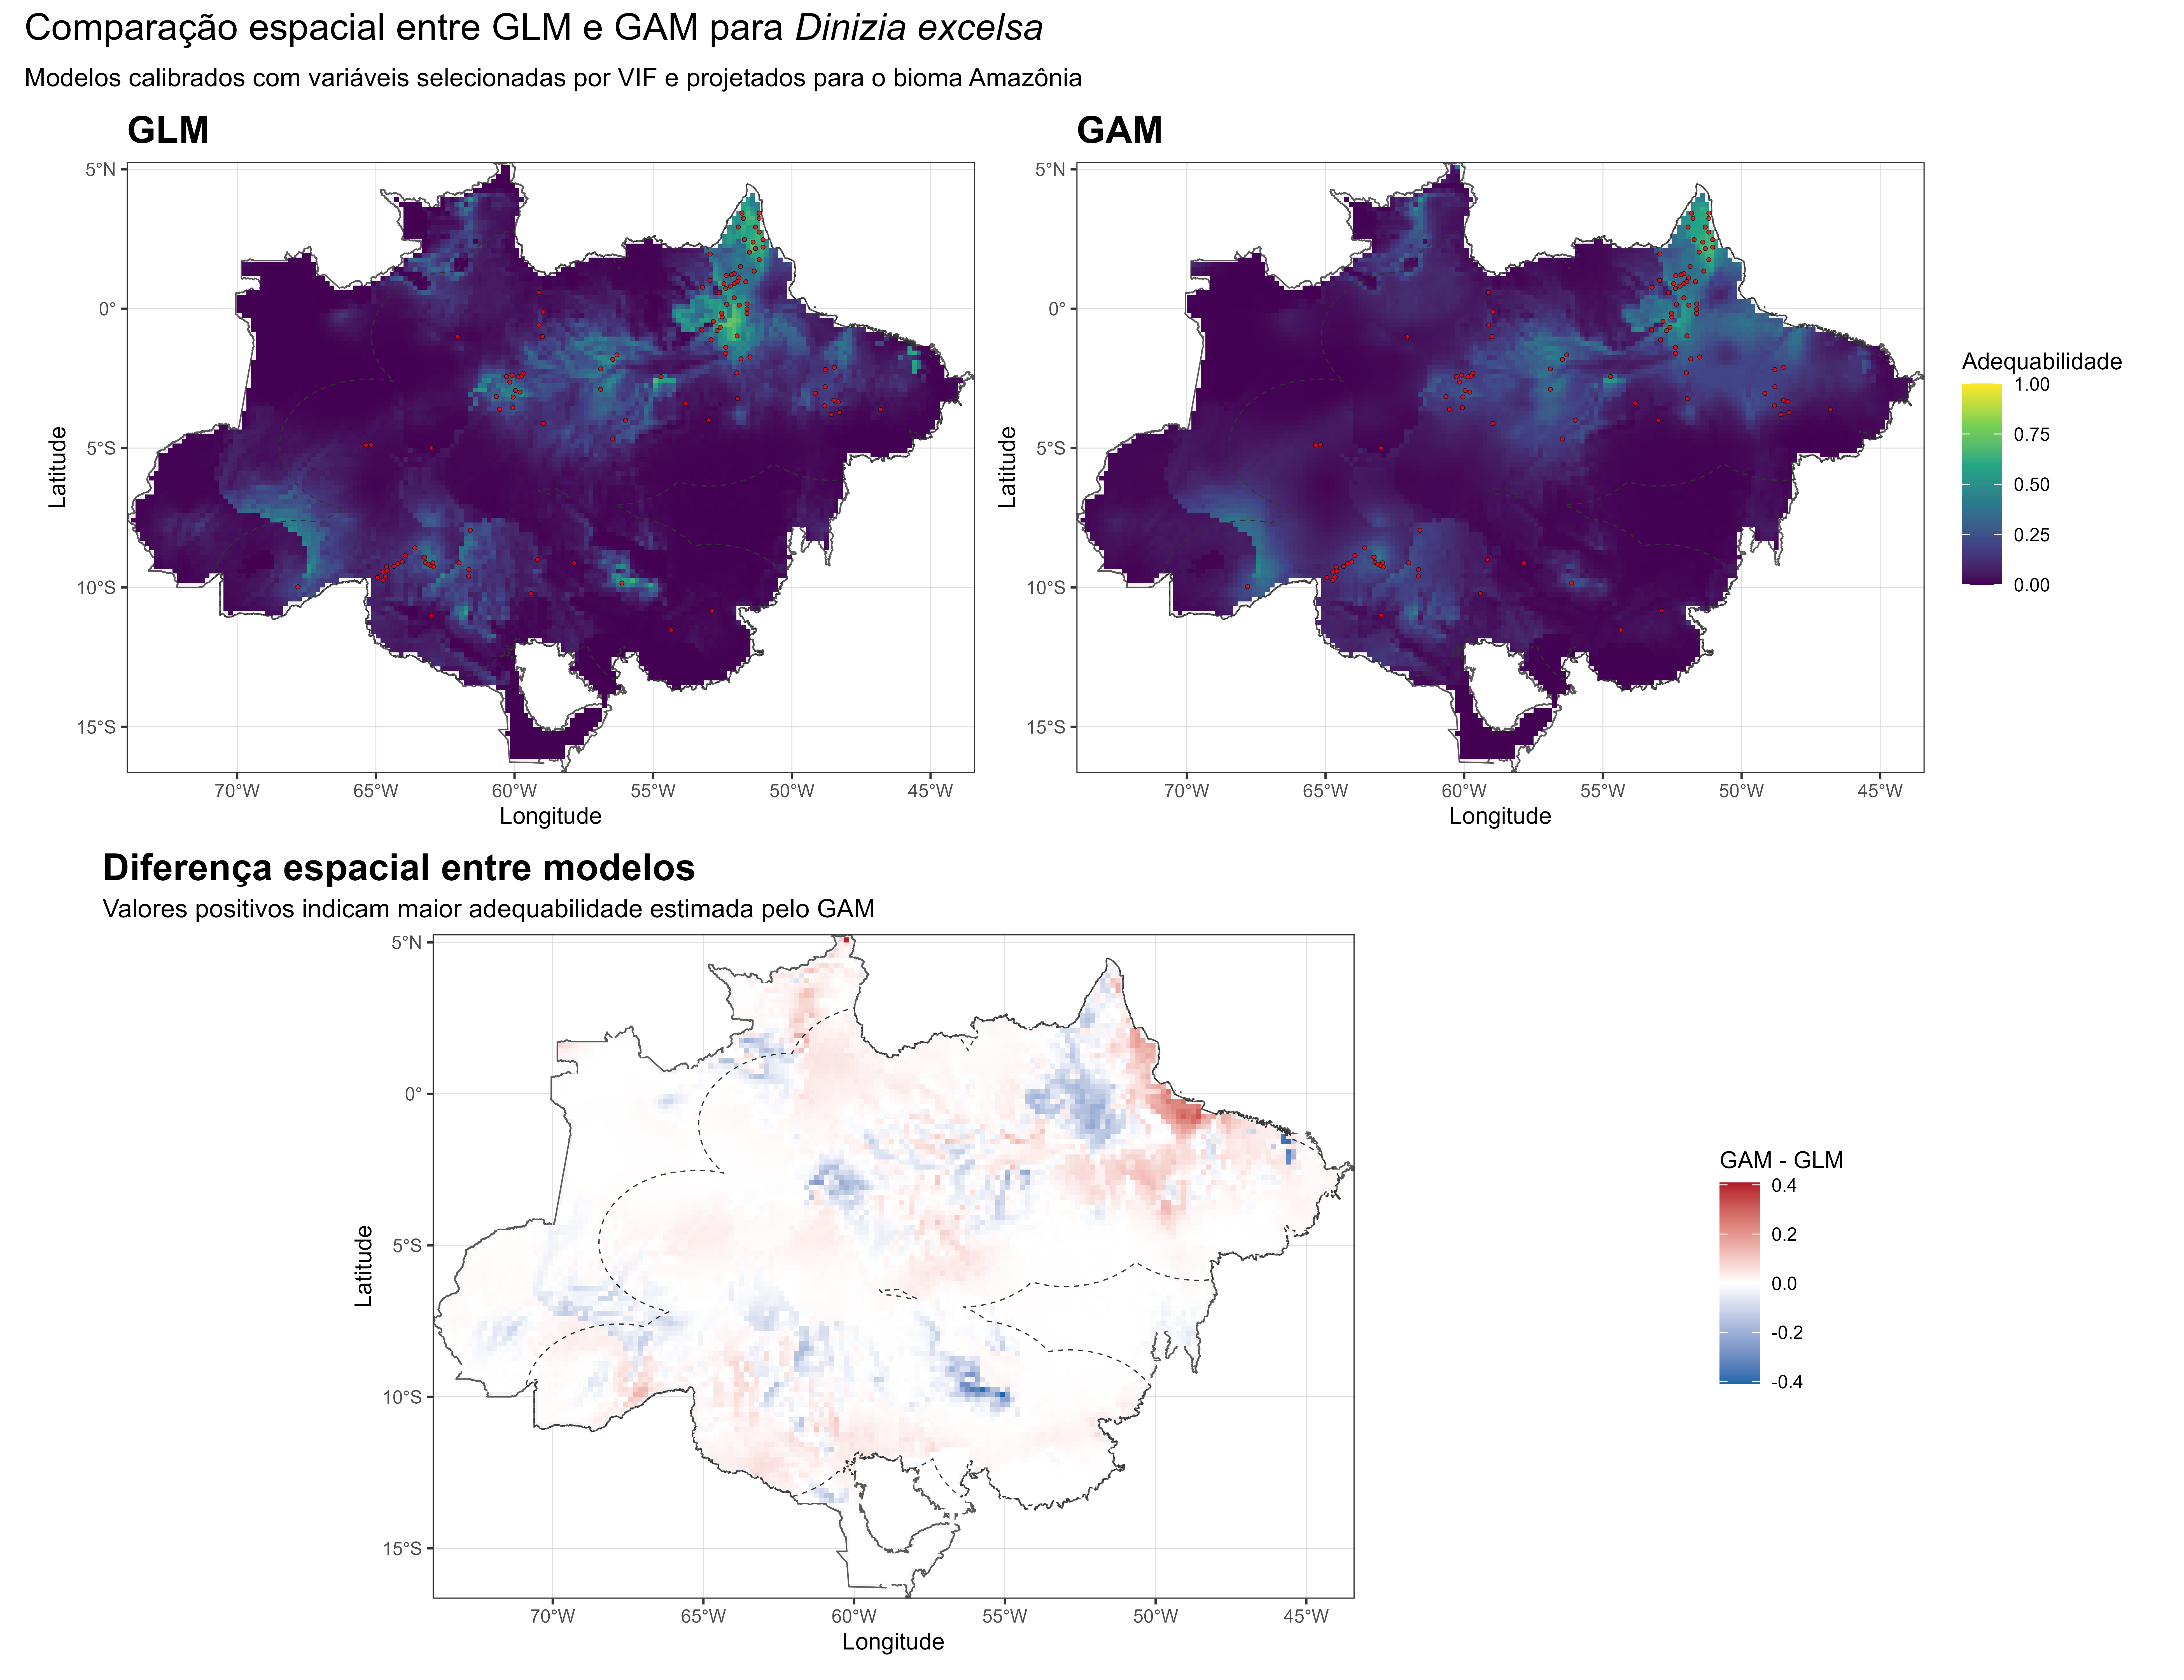
\includegraphics[width=0.96\textwidth]{figuras/unidade07/unidade07_comparacao_glm_gam.png}
	\caption{Comparação entre mapas de adequabilidade estimados por GLM e GAM para \textit{Dinizia excelsa}.}
	\label{fig:unidade07_comparacao_glm_gam}
\end{figure}

\section{Pipeline completo}

\rscriptfile{scripts/unidade07/08_pipeline_gam.R}

\section{Síntese da unidade}

O GAM representa uma etapa intermediária entre modelos paramétricos simples e algoritmos de aprendizado de máquina. Ele mantém boa interpretabilidade, mas permite capturar relações ambientais não lineares. Para \textit{Dinizia excelsa}, o GAM permite visualizar respostas ecológicas flexíveis aos gradientes ambientais selecionados.

\begin{conceito}[title={\faBook\quad Mensagem central}]
	O GAM é especialmente útil quando se espera que a espécie responda de forma não linear aos gradientes ambientais. Em SDM, ele oferece um equilíbrio entre flexibilidade, interpretação ecológica e desempenho preditivo.
\end{conceito}

\section{Exercícios de fixação}

\begin{enumerate}
	\item Explique a diferença entre GLM e GAM.
	\item O que representa uma função suave em um GAM?
	\item Por que o parâmetro \(k\) deve ser escolhido com cautela?
	\item Explique por que GAMs podem capturar respostas ecológicas não lineares.
	\item O que significa sobreajuste em SDM?
	\item Como curvas de resposta parcial ajudam na interpretação ecológica?
	\item Compare vantagens e limitações de GLM e GAM em SDM.
\end{enumerate}

% ============================================================
% UNIDADE 8
% ============================================================

